% --------- document setup ---------
\documentclass[12pt]{article}
\usepackage[
    left=1in,
    right=1in,
    top=0.5in,
    bottom=0.5in,
    includehead,
    includefoot
]{geometry}
\setlength{\parskip}{0.75em} % larger jumps at end of paragraph
\setlength{\parindent}{0pt} % no indent
\pagenumbering{gobble} % no page numbers

% --------- packages ---------
\usepackage{graphicx} % required for inserting images
\usepackage{multicol} % two column feature
\usepackage{hyperref} % hyperlinks
\usepackage{etoolbox} % if-then-else logic
\usepackage{amsmath, amsfonts, amssymb, amsthm, mathrsfs} % math
\usepackage{float} % figure env
\usepackage{tikz} % drawing things
\usetikzlibrary{automata, positioning}
\usepackage{xcolor} % colors
\usepackage[most]{tcolorbox} % answer boxes
\usepackage{fancyhdr} % header
\usepackage{fancyvrb} % fancy verbatim
\usepackage{ifthen} % conditional statements
\usepackage{lipsum} % filler text
\usepackage{xstring} % For string manipulation
\usepackage{enumitem} % for hint hanging indent
\usepackage{outlines} % for outlines
\usepackage{fancybox} % for nice title page box
\usepackage{soul} % for strikethrough
\usepackage{algorithm} % for algorithms
\usepackage{dsfont}

\newcommand{\note}[1]{{\footnotesize
        \begin{description}
                [leftmargin=3.4em,style=nextline]
            \item[Note:] {#1}
        \end{description}}
}

% --------- Header + Title ---------
\renewcommand\maketitle{
    \begin{center}
        \shadowbox{\parbox{5.3in}{{\small {\bf {\sc Georgia Tech Spring 2025
                \hfill CS 3511: Honors Algorithms}}}
                \medbreak
                \begin{center}
                    {\large \bfseries \reportTitle}
                \end{center}
                \medbreak
                Authors: {\em \authors}
                \newline
                Date: \reportDate
            \vspace{2pt}}
        }
        \vspace{6pt}
    \end{center}
}

% --------- Custom symbols ---------
\newcommand{\C}{\mathbb{C}}
\newcommand{\E}{\mathbb{E}}
\newcommand{\F}{\mathbb{F}}
\newcommand{\N}{\mathbb{N}}
\renewcommand{\P}{\mathbb{P}}
\newcommand{\Q}{\mathbb{Q}}
\newcommand{\R}{\mathbb{R}}
\newcommand{\Z}{\mathbb{Z}}
\newcommand{\Var}{\operatorname{Var}}
\newcommand{\bigO}{\mathcal{O}}
\newcommand{\Ptime}{\mathrm{P}}
\newcommand{\NPtime}{\mathrm{NP}}
\newcommand{\poly}{\text{poly}}
\newcommand{\Alg}{\mathcal{A}}
\newcommand{\Opt}{\operatorname{OPT}}
\newcommand{\dx}{\ensuremath{\mathrm{d}x}}
\newcommand{\floor}[1]{\left\lfloor #1 \right\rfloor} % for floor
\newcommand{\ceil}[1]{\left\lceil #1 \right\rceil} % for ceiling

% ------------ Document ------------
\begin{document}

\newcommand{\reportTitle}{Final Project}
\newcommand{\reportDate}{Wednesday 4/16/25}

\newcommand{\authors}{Arjun Sheshadri, Vilohith Gokarakonda, Yiqi Sun, Tyler Huang}

\maketitle

\section{Introduction}

Suppose if you have a graph $G = (V, E)$ with a given adjacency matrix, which represents where any two nodes are connected to each other. Suppose you wanted to find the shortest path to one node, using all nodes as a starting point.

Shortest distances between all pairs of nodes in a graph is important for its real world applications in communication networks, social graphs, and more. Edges in such graphs can be added and removed at any time, so being able to efficiently maintain all pairs distances is crucial. Using the Floyd-Warshall Algorithm, we are able to accomplish this in $\bigO(n^3)$ time. However, this becomes inefficient for larger or frequently changing graphs.

This report explores a \textit{dynamic algorithm} described in Jan van den Brand's \href{https://www.dropbox.com/scl/fi/zjfbk8dbxbzcn05dr8l11/fall22_daa_lecturenotes.pdf?rlkey=g6z7z1hvj7jknvlpy1s3dqcjw&e=1&st=13r18doq&dl=0}{notes} for maintaining All-Pairs-Shortest-Paths (\texttt{APSP}) in directed graphs with or without edge weights. Instead of recalculating shortest distances from scratch every update, it efficiently maintains a data structure where all distances can be updated in $\displaystyle \tilde \bigO(n^{2.5})$ time when an edge to a single vertex is added or removed. Specifically, it uses concepts from dynamic algebraic algorithms, involving polynomial matrix inverses to represent path information, and extending them to full distances with random sampling and Dijkstra's algorithm.

In this report, we present the problem statement, and the technical background relevant to the paper, including ring algebra, polynomial matrices, and how edges are updated. We also cover the steps to the solution, and connect this approach to the original groundbreaking \href{https://www.dropbox.com/scl/fi/5w4k0lg0u8e36zugapp6c/Sankowski-COCOON-05-subquadratic-dynamic-distances.pdf?rlkey=5eahwsl7a49kwxyvlr7yqyoz3&e=2&st=d3zo7owc&dl=0}{paper} by Sankowski, which can do updates in $\displaystyle \tilde \bigO(n^{1.932})$  randomized time and queries in $\displaystyle \tilde \bigO(n^{1.288})$ randomized time. Specifically, we compare their mathematical foundations, update operations, applications, and time complexities.

\section{Problem Statement}

Given a graph $G(V, E)$, we want to develop a data structre that can maintain \texttt{APSP} dynamically with an initial overhead $\displaystyle \tilde \bigO(n^{3.5})$ time and supports queries and updates in $\displaystyle \tilde \bigO(n^{2.5})$ time. Since this algorithm is optimized for maintaining \texttt{APSP} for changing graphs (hence requires a dynamic algorithm), having a time complexity of $\displaystyle \tilde \bigO(n^{2.5})$ is more efficient compared to the naive approach which takes $\bigO(n^3)$ time for queries and updates.

\newpage

Specifically, we will be working towards proving the following theorem:

\textbf{Theorem 1.0.0}: \emph{There exists a data structure that supports the following operations}:
\begin{enumerate}
    \item \textsc{Initialize($G = (V, E)$)} \emph{Initialize an $n$-node graph and return \texttt{APSP} in $\displaystyle \tilde \bigO(n^{3.5})$ time.}
    \item \textsc{Update($v,\,E^+,\,E^-$)} \emph{Given a vertex $v$ and two sets of edges $E^+\subseteq(\{v\}\times V\cup V\times\{v\})$ to insert and $E^-$ to delete (all incident to $v$), update $G$ and return the new \texttt{APSP} in $\displaystyle \tilde \bigO(n^{2.5})$ time.}
\end{enumerate}

Additionally, we will be extending this theorem using Sankowski's paper:

\textbf{Theorem 1.0.1}: \emph{There exists a data structure that supports the following operations}:
\begin{enumerate}
    \item \textsc{Initialize($G = (V, E)$)} \emph{Preprocess in $\displaystyle \tilde \bigO(n^{3})$ time.}
    \item \textsc{Update($e$)} \emph{Insert or delete a single edge $e\in V\times V$ in $\bigO(n^{1.932})$ randomized time.}
    \item \textsc{Query($s, t$)} \emph{Return the current distance $\mathrm{dist}_G(s,t)$ in $\bigO(n^{1.288})$ randomized time.}
\end{enumerate}
\emph{All operations succeed with high probability over the random choices.}

We will be covering general overviews of topics that help toward understanding the intuition behind these theorems in the next section.

\section{Technical Background}

\subsection{Matrix Multiplication Recap and Naive APSP}

Matrix multiplication is an important concept that we will be making extensive use of to understand the technical components in this report. You are already familiar with the basic method of multiplying two matrices with the same inner dimension, where you multiply the $n$-th row of the first matrix with the $n$-th column of the second matrix. Below is a visual representation:

\[
    \begin{bmatrix}
        a & b \\
        c & d
    \end{bmatrix}
    \begin{bmatrix}
        e & f \\
        g & h
    \end{bmatrix}
    =
    \begin{bmatrix}
        a \cdot e + b \cdot g & a \cdot f + b \cdot h \\
        c \cdot e + d \cdot g & c \cdot f + d \cdot h
    \end{bmatrix}
\]

Notice how in each $(i, j)$ entry of the product matrix, we compute the \emph{dot product} of the vector that forms the $i$-th row of the first matrix and the $j$-th column of the second matrix. The \emph{dot product} is simply an operation on the entries of two vectors involving the typical $+$ and $\times$ operations.

Let's take a quick detour from matrix multiplication to talk about the well-known Floyd-Warshall algorithm for computing \texttt{APSP}. The key realization to understanding this algorithm is that between some start node $s$ and some terminal node $t$, the shortest path from $s \to t$ is the shorter path we can get from directly travelling from $s \to t$ vs. the path we get by travelling from $s$ to some intermediate node $k$ and then from $k$ to $t$. For a visualization, consider the trivial example below:

\begin{center}
    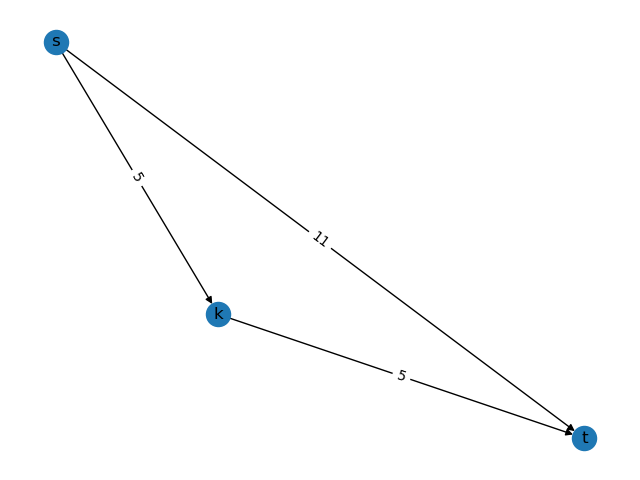
\includegraphics[scale=0.5]{media/Figure_1.png}
\end{center}

In the above graphic, the direct path from $s \to t$ has a cost of 11, while the path from $s \to k$ has a cost of 5 and the path from $k \to t$ has a cost of 5 as well. We can see that if we take $\min \{\mathrm{dist}_{s,t} = 11, \mathrm{dist}_{s,k} + \mathrm{dist}_{k,t} = 10 \}$, we get that by considering the intermediate node $k$, we arrive at a cheaper path from $s$ to $t$.

How does the above logic tie into matrix multiplication? Well, it might be intutive to think of graphs in terms of adjacency matricies and the core Floyd-Warshall computation as a dot product between some vector $u$ that represents the shortest known paths from the starting node $s$ to all possible intermediate nodes $k$, and another vector $v$ that represents the shortest paths from all possible intermediate nodes $k$ to the terminal node $t$.

For those already familiar with computing the shortest path between some start node $s$ and some terminal node $t$ on a directed and optionally weighted graph, it might be intuitive to also represent the calculation in terms of a dot product. Suppose some vector $v$ corresponds to the to the best known path costs from $s$ to every other node $t$ in the graph, and the index of an element in $v$ corresponds to the node $t$ that that element represents. An example of $v$ may be the following

\[
    v =
    \begin{bmatrix}
        1 & 2 & 5 & 7 & 0 & 10
    \end{bmatrix}
\]

\subsection{Abstract Algebra Overview and Ring Operations}
\subsection{Polynomial Matrices}
\subsection{Edge Updates}
\subsection{Hitting Sets}

\section{Solution}
\subsection{Algorithm}
\subsection{Time Complexity Analysis}

\section{Extension and Comparison}
\subsection{Broader Algebraic Structures}
\subsection{General Update Query}
\subsection{Multiple Matrix Functions}
\subsection{Better Complexity Bounds}

\section*{References}

\begin{enumerate}
    \item \href{https://www.dropbox.com/scl/fi/zjfbk8dbxbzcn05dr8l11/fall22_daa_lecturenotes.pdf?rlkey=g6z7z1hvj7jknvlpy1s3dqcjw&e=1&st=13r18doq&dl=0}{Jan van den Brand's Notes}
    \item \href{https://www.dropbox.com/scl/fi/5w4k0lg0u8e36zugapp6c/Sankowski-COCOON-05-subquadratic-dynamic-distances.pdf?rlkey=5eahwsl7a49kwxyvlr7yqyoz3&e=2&st=d3zo7owc&dl=0}{Sankowski's Paper}
\end{enumerate}

\end{document}
